%%%%%%%%%%%%%%%%%%%%%%%%%%%%%%%%%%%%%%%%%%%%%%%%%%%%%%%%%%%%%%%%%%%%%%%%%%%%
%
% profiling.tex
%
% Thomas Heitz, 23/10/2009
%
% $Id$
%
%%%%%%%%%%%%%%%%%%%%%%%%%%%%%%%%%%%%%%%%%%%%%%%%%%%%%%%%%%%%%%%%%%%%%%%%%%%%

%%%%%%%%%%%%%%%%%%%%%%%%%%%%%%%%%%%%%%%%%%%%%%%%%%%%%%%%%%%%%%%%%%%%%%%%%%%%
\chapt[chap:profiling]{Profiling Processing Resources}
\markboth{Profiling Processing Resources}{Profiling Processing Resources}
%%%%%%%%%%%%%%%%%%%%%%%%%%%%%%%%%%%%%%%%%%%%%%%%%%%%%%%%%%%%%%%%%%%%%%%%%%%%

%%%%%%%%%%%%%%%%%%%%%%%%%%%%%%%%%%%%%%%%%%%%%%%%%%%%%%%%%%%%%%%%%%%%%%%%%%%%
\sect[sec:profiling:overview]{Overview}
%%%%%%%%%%%%%%%%%%%%%%%%%%%%%%%%%%%%%%%%%%%%%%%%%%%%%%%%%%%%%%%%%%%%%%%%%%%%

This is a reporting tool for GATE processing resources. It reports the
total time taken by processing resources and the time taken for each
document to be processed by an application of type corpus pipeline.

GATE use log4j, a logging system, to write profiling informations in a
file. The GATE profiling reporting tool uses the file generated by log4j and
produces a report on the processing resources. It profiles JAPE grammars at
the rule level, enabling the user precisely identify the
performance bottlenecks. It also produces a report on the time taken to
process each document to find problematic documents.

This initial code for the reporting tool was written by Intelius employees
Andrew Borthwick and Chirag Viradiya and generously released under the LGPL
licence to be part of GATE.

\begin{figure}[htbp]
\begin{center}
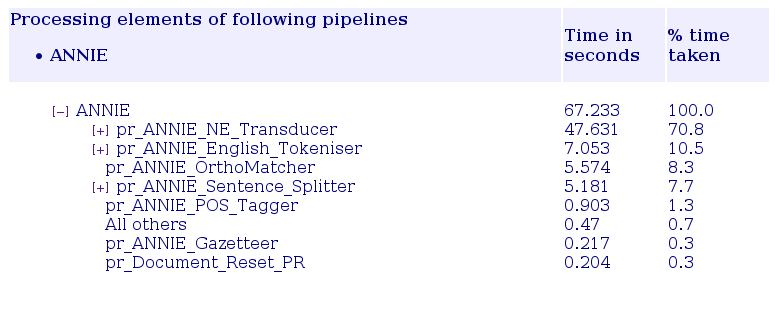
\includegraphics[width=14cm]{profiling-report.png}
\end{center}
\caption{Example of HTML profiling report for ANNIE}
\label{fig:profiling-report}
\end{figure}

%%%%%%%%%%%%%%%%%%%%%%%%%%%%%%%%%%%%%%%%%%%%%%%%%%%%%%%%%%%%%%%%%%%%%%%%%%%%
\subsection{Features}

\begin{itemize}
  \item Ability to generate the following two reports
  \begin{itemize}
    \item Report on processing resources. For each level of processing:
    application, processing resource (PR) and grammar rule, subtotalled at each
    level.
    \item Report on documents processed. For some or all PR,
    sorted in decreasing processing time.
  \end{itemize}

  \item Report on processing resources specific features
  \begin{itemize}
    \item Sort order by time or by execution.
    \item Show or hide processing elements which took 0 milliseconds.
    \item Generate HTML report with a collapsible tree.
  \end{itemize}

  \item Report on documents processed specific features
  \begin{itemize}
    \item Limit the number of document to show from the most time consuming.
    \item Filter the PR to display statistics for.
  \end{itemize}

  \item Features common to both reports
  \begin{itemize}
    \item Generate report as indented text or in HTML format.
    \item Generate a report only on the log entries from the last logical
    run of GATE.
    \item All processing times are reported 
    in milliseconds and in terms of percentage (rounded to nearest 
    0.1\%) of total time.
    \item Command line interface and API.
    \item Detect if the benchmark.txt file is modified while generating
    the report. 
  \end{itemize}
\end{itemize}

%%%%%%%%%%%%%%%%%%%%%%%%%%%%%%%%%%%%%%%%%%%%%%%%%%%%%%%%%%%%%%%%%%%%%%%%%%%%
\subsection{Limitations}

Be aware that the profiling doesn't support non corpus pipeline as
application type. There is indeed no interest in profiling a non corpus
pipeline that works on one or no document at all. To get meaningful results
you should run your corpus pipeline on at least 10 documents.

%%%%%%%%%%%%%%%%%%%%%%%%%%%%%%%%%%%%%%%%%%%%%%%%%%%%%%%%%%%%%%%%%%%%%%%%%%%%
\sect[sec:profiling:gui]{Graphical User Interface}
%%%%%%%%%%%%%%%%%%%%%%%%%%%%%%%%%%%%%%%%%%%%%%%%%%%%%%%%%%%%%%%%%%%%%%%%%%%%

The activation of the profiling and the creation of profiling reports are
accessible from the `Tools' menu in GATE with the submenu `Profiling
Reports'.

You can `Start Profiling Applications' and `Stop Profiling Applications' at
any time. The logging is cumulative so if you want to get a new report you
must use the `Clear Profiling History' menu item when the profiling is stopped.

Be very careful that you must start the profiling before you load your
application or you will need to reload every Processing Resource that uses a
Transducer. Otherwise you will get an Exception similar to:

\begin{small}
\begin{verbatim}
java.lang.IndexOutOfBoundsException: Index: 2, Size: 0
	at java.util.ArrayList.RangeCheck(ArrayList.java:547)
	at java.util.ArrayList.get(ArrayList.java:322)
	at gate.jape.SinglePhaseTransducer.updateRuleTime(SinglePhaseTransducer.java:678)
\end{verbatim}
\end{small}

Two types of reports are available: `Report on Processing Resources' and
`Report on Documents Processed'. See the previous section for more
information.

%%%%%%%%%%%%%%%%%%%%%%%%%%%%%%%%%%%%%%%%%%%%%%%%%%%%%%%%%%%%%%%%%%%%%%%%%%%%
\sect[sec:profiling:cli]{Command Line Interface}
%%%%%%%%%%%%%%%%%%%%%%%%%%%%%%%%%%%%%%%%%%%%%%%%%%%%%%%%%%%%%%%%%%%%%%%%%%%%

\paragraph{Report on processing resources}

\par Usage: java gate.util.reporting.PRTimeReporter [Options]
\par Options: 
\par -i input file path (default: benchmark.txt in the user's .gate
directory\footnote{GATE versions up to 5.2 placed benchmark.txt in the
execution directory.})
\par -m print media - html/text (default: html)
\par -z suppressZeroTimeEntries - true/false (default: true)
\par -s sorting order - exec\_order/time\_taken (default: exec\_order)
\par -o output file path (default: report.html/txt in the system temporary directory)
\par -l logical start (not set by default)
\par -h show help
\\

\textit{Note that suppressZeroTimeEntries will be ignored if the
sorting order is `time\_taken'}

\paragraph{Report on documents processed}

\par Usage: java gate.util.reporting.DocTimeReporter [Options]
\par Options: 
\par -i input file path (default: benchmark.txt in the user's .gate
directory\footnote{GATE versions up to 5.2 placed benchmark.txt in the
execution directory.})
\par -m print media - html/text (default: html)
\par -d number of docs, use -1 for all docs (default: 10 docs)
\par -p processing resource name to be matched (default: all\_prs)
\par -o output file path (default: report.html/txt in the system temporary directory)
\par -l logical start (not set by default)
\par -h show help

\paragraph{Examples}

\begin{itemize}
  \item Run report 1: Report on 
  Total time taken by each processing element across corpus
  \begin{itemize}
    \item java -cp "gate/bin:gate/lib/GnuGetOpt.jar" 
    gate.util.reporting.PRTimeReporter -i benchmark.txt 
    -o report.txt -m text
  \end{itemize}
  \item Run report 2: Report on Time 
  taken by document within given corpus.
  \begin{itemize}
    \item java -cp "gate/bin:gate/lib/GnuGetOpt.jar" 
    gate.util.reporting.DocTimeReporter -i benchmark.txt
    -o report.html -m html
  \end{itemize}
\end{itemize}

%%%%%%%%%%%%%%%%%%%%%%%%%%%%%%%%%%%%%%%%%%%%%%%%%%%%%%%%%%%%%%%%%%%%%%%%%%%%
\sect[sec:profiling:api]{Application Programming Interface}
%%%%%%%%%%%%%%%%%%%%%%%%%%%%%%%%%%%%%%%%%%%%%%%%%%%%%%%%%%%%%%%%%%%%%%%%%%%%

%%%%%%%%%%%%%%%%%%%%%%%%%%%%%%%%%%%%%%%%%%%%%%%%%%%%%%%%%%%%%%%%%%%%%%%%%%%%
\subsection{Log4j.properties}

This is required to direct the profiling information to the benchmark.txt
file. The benchmark.txt generated by GATE will be used as input for GATE
profiling report tool as input.

\begin{itemize}
  \item \# File appender that outputs only benchmark messages
  \item log4j.appender.benchmarklog=org.apache.log4j.RollingFileAppender
  \item log4j.appender.benchmarklog.Threshold=DEBUG
  \item log4j.appender.benchmarklog.File=\${user.home}/.gate/benchmark.txt
  \item log4j.appender.benchmarklog.MaxFileSize=5MB
  \item log4j.appender.benchmarklog.MaxBackupIndex=1
  \item log4j.appender.benchmarklog.layout=org.apache.log4j.PatternLayout
  \item log4j.appender.benchmarklog.layout.ConversionPattern=\%m\%n
  \item \# Configure the Benchmark logger so that it only goes to the
  benchmark log file
  \item log4j.logger.gate.util.Benchmark=DEBUG, benchmarklog
  \item log4j.additivity.gate.util.Benchmark=false
\end{itemize}


%%%%%%%%%%%%%%%%%%%%%%%%%%%%%%%%%%%%%%%%%%%%%%%%%%%%%%%%%%%%%%%%%%%%%%%%%%%%
\subsection{Benchmark log format}

The format of the benchmark file that logs the times is as follow:

\begin{small}\begin{verbatim}
timestamp START PR_name
timestamp duration benchmarkID class features
timestamp duration benchmarkID class features
...
\end{verbatim}\end{small}

with the timestamp being the difference, measured in milliseconds, between the current time and midnight, January 1, 1970 UTC.

Example:

\begin{small}\begin{verbatim}
1257269774770 START Sections_splitter
1257269774773 0 Sections_splitter.doc_EP-1026523-A1_xml_00008.documentLoaded
gate.creole.SerialAnalyserController
{corpusName=Corpus for EP-1026523-A1.xml_00008,
documentName=EP-1026523-A1.xml_00008}
...
\end{verbatim}\end{small}

%%%%%%%%%%%%%%%%%%%%%%%%%%%%%%%%%%%%%%%%%%%%%%%%%%%%%%%%%%%%%%%%%%%%%%%%%%%%
\subsection{Enabling profiling}

There are two ways to enable profiling of the processing resources:

\begin{enumerate}
  \item In gate/build.properties, add the line:
run.gate.enable.benchmark=true

  \item In your Java code, use the method:
Benchmark.setBenchmarkingEnabled(true)
\end{enumerate}

%%%%%%%%%%%%%%%%%%%%%%%%%%%%%%%%%%%%%%%%%%%%%%%%%%%%%%%%%%%%%%%%%%%%%%%%%%%%
\subsection{Reporting tool }

\paragraph*{Report on processing resources}

\begin{enumerate}
  \item Instantiate the Class PRTimeReporter
  \begin{enumerate}
    \item PRTimeReporter report = new PRTimeReporter();
  \end{enumerate}
  \item Set the input benchmark file
  \begin{enumerate}
    \item File benchmarkFile = new File("benchmark.txt");
    \item report.setBenchmarkFile(benchmarkFile);
  \end{enumerate}
  \item Set the output report file
  \begin{enumerate}
    \item File reportFile = new File("report.txt");
    or
    \item File reportFile = new File("report.html");
    \item report.setReportFile(reportFile); 
  \end{enumerate}
  \item Set the output format:
    in html or text format (default: MEDIA\_HTML)
  \begin{enumerate}
    \item report.setPrintMedia(PRTimeReporter.MEDIA\_TEXT);
    or
    \item report.setPrintMedia(PRTimeReporter.MEDIA\_HTML);
  \end{enumerate}
  \item Set the sorting order: Sort in order 
    of execution or descending order of time taken (default: EXEC\_ORDER)
  \begin{enumerate}
    \item report.setSortOrder(PRTimeReporter.SORT\_TIME\_TAKEN); 
    or
     \item report.setSortOrder(PRTimeReporter.SORT\_EXEC\_ORDER);
  \end{enumerate}
  \item Set if suppress zero time entries:
    True/False (default: True). Parameter ignored if SortOrder specified 
    is `SORT\_TIME\_TAKEN'
  \begin{enumerate}
    \item report.setSuppressZeroTimeEntries(true);
  \end{enumerate}
  \item Set the logical start: A string indicating 
    the logical start to be operated upon for generating reports
  \begin{enumerate}
    \item report.setLogicalStart("InteliusPipelineStart");
  \end{enumerate}
  \item Generate the text/html report
  \begin{enumerate}
    \item report.executeReport();
  \end{enumerate}
\end{enumerate}

\paragraph*{Report on documents processed}

\begin{enumerate}
  \item Instantiate the Class DocTimeReporter
  \begin{enumerate}
    \item DocTimeReporter report = new DocTimeReporter();
  \end{enumerate}
  \item Set the input benchmark file
  \begin{enumerate}
    \item File benchmarkFile = new File("benchmark.txt");
    \item report.setBenchmarkFile(benchmarkFile);
  \end{enumerate}
  \item Set the output report file
  \begin{enumerate}
    \item File reportFile = new File("report.txt");
    or
    \item File reportFile = new File("report.html");
    \item report.setReportFile(reportFile); 
  \end{enumerate}
  \item Set the output format: Generate report 
    in html or text format (default: MEDIA\_HTML)
  \begin{enumerate}
    \item report.setPrintMedia(DocTimeReporter.MEDIA\_TEXT); 
    or
    \item report.setPrintMedia(DocTimeReporter.MEDIA\_HTML); 
    \end{enumerate}
  \item Set the maximum number of documents: Maximum number of documents 
    to be displayed in the report (default: 10 docs)
  \begin{enumerate}
    \item report.setNoOfDocs(2); 
    // 2 docs or
    \item report.setNoOfDocs(DocTimeReporter.ALL\_DOCS); 
    // All documents
    \end{enumerate}
  \item Set the PR matching regular expression: A PR name or a regular
    expression to filter the results (default: MATCH\_ALL\_PR\_REGEX).
  \begin{enumerate}
    \item report.setSearchString("HTML"); 
    // match ALL PRS having HTML as substring
    \end{enumerate}
  \item Set the logical start: A string indicating 
    the logical start to be operated upon for generating reports
  \begin{enumerate}
    \item report.setLogicalStart("InteliusPipelineStart");
  \end{enumerate}
  \item Generate the text/html report
  \begin{enumerate}
    \item report.executeReport();
   \end{enumerate}
\end{enumerate}
